\documentclass[../tesis_main_file.tex]{subfiles}
\begin{document}
\onlyinsubfile{\graphicspath{ {../figuras/} }}
\onlyinsubfile{\pagenumbering{arabic}}
\onlyinsubfile{\setcounter{chapter}{1}}
\onlyinsubfile{\chapter{Inestabilidad de dos corrientes}}
\section{Introducción}
Para tratar el tema de inestabilidades se mostrará primero que frecuencias complejas pueden aparecer en el plasma si se tiene un arreglo de haces de partículas adecuado \cite{bellan2008fundamentals}.\\
%The first part of this chapter develops some
%preparatory ideas by showing that complex frequencies, i.e., wave instabilities,
%can develop if there are suitably arranged particle beams in a plasma.
El tratatamiento inicial se hará desde la perspectiva de fluidos. Se parte entonces de las siguientes ecuaciones:
\begin{equation}
\label{cont_nl}
\frac{\partial n_{\sigma}}{\partial t} + \overrightarrow{\nabla} \cdot n_{\sigma}\overrightarrow{\textbf{u}}_{\sigma}=0
\end{equation}
\begin{equation}
\label{eq_movimiento_nl}
n_{\sigma}m_{\sigma}\frac{d\overrightarrow{\textbf{u}}_{\sigma}}{dt}= n_{\sigma}q_{\sigma}(\overrightarrow{\textbf{E}} + \overrightarrow{\textbf{u}}_{\sigma} \times \overrightarrow{\textbf{B}}) - \nabla P_{\sigma} - \textbf{R}_{\sigma \alpha}
\end{equation}
\begin{equation}
\label{poisson_nl}
\nabla ^2 \Phi = -\frac{1}{\epsilon_0}\sum _{\sigma}q_{\sigma} n_{\sigma}
\end{equation}
Las cuales son respectivamente la ecuación de continuidad, movimiento y Poisson para cada especie. Al tratarse del caso electróstatico la ecuación \ref{eq_movimiento_nl} se puede reducir a la siguiente forma:
\begin{equation}
\label{eq_mov_simpl_nl}
n_{\sigma}m_{\sigma}\frac{d\overrightarrow{\textbf{u}}_{\sigma}}{dt}= n_{\sigma}q_{\sigma} \overrightarrow{\textbf{E}}
\end{equation}
Con $\overrightarrow{\textbf{E}} = - {\overrightarrow\nabla} \Phi$. Y donde se han despreciado los términos de aceleración debido al campo magnético (puesto que ese término es cero para modos longitudinales), la presión y a la fuerza de fricción debida a colisiones. Además, se tiene $d/dt \equiv \partial / \partial t + \overrightarrow{\textbf{u}}_{\sigma} \cdot \overrightarrow{\nabla}$, la cual se le conoce como la derivada convectiva.\\
%Los términos $\nabla P_{\sigma}$ y $\textbf{R}_{\sigma \alpha}$ se refieren a la presión y a la fuerza de fricción resultante de las colisiones entre las especies $\sigma$ y $\alpha$ respectivamente.\\
El siguiente paso entonces es introducir un método que permita ver el comportamiento de las ondas longitudinales en el  plasma debido a cada una de las especies. Dicho método se le conoce como análisis lineal y el procedimiento es el siguiente:
\begin{itemize}
\item Se reduce el sistema a un simple conjunto de ecuaciones que describan su comportamiento.
\item Se determina una solución de equilibrio para las ecuaciones y a las cantidades de equilibrio se les designa con el subíndice 0, indicando que son cantidades de orden cero.
\item Si $\lbrace f(\textbf{x},t), g(\textbf{x},t),h(\textbf{x},t),...\rbrace$ es el conjunto de las variables dependientes y se le agrega una perturbación a una de las variables, entonces al resolver el sistema de ecuaciones se obtendrá la respuesta de las otras variables a la perturbación. Supongasé que se le agrega una perturbación $\epsilon f_1$ a la variable $f$, con $\epsilon \ll 1$ entonces se tiene:
\begin{equation*}
f = f_0 + \epsilon f_1
\end{equation*}
El sistema entonces da la dependencia funcional de las otras variables, por ejemplo $g = g(f) = g(f_0 + \epsilon f_1)$. Dado que ésta dependencia por lo general es no lineal la expansión de Taylor da $g = g_0 + \epsilon g_1 + \epsilon^2 g_2 + \epsilon^3 g_3 +...$ Si se considera a las epsilons como coeficientes implícitos las variables se pueden escribir entonces como:
$$
\begin{array}{lllllllll}
f &= &f_0 &+ &f_1 \\
g &= &g_0 &+ &g_1 &+ &g_2 &+ &...\\
h &= &h_0 &+ &h_1 &+ &h_2 &+ &...
\end{array}
$$
\item Se reescriben entonces las ecuaciones del sistema con las variables expandidas a primer orden y se discriminan los términos de segundo orden resultantes, así como también haciendo uso de las soluciones de equilibrio para simplificar las expresiones.
\end{itemize}
Para el caso de la ecuación de continuidad se tiene entonces:
\begin{equation}
\frac{\partial (n_{\sigma 0} + n_{\sigma 1})}{\partial t} + \overrightarrow{\nabla} \cdot [(n_{\sigma 0}+n_{\sigma 1})(\overrightarrow{\textbf{u}}_{\sigma 0} + \overrightarrow{\textbf{u}}_{\sigma 1})]=0
\end{equation}
Donde la solución de equiibrio es:
\begin{equation}
\frac{\partial n_{\sigma 0}}{\partial t} + \overrightarrow{\nabla} \cdot n_{\sigma 0}\overrightarrow{\textbf{u}}_{\sigma 0}=0
\end{equation}
Lo que da:
\begin{equation}
\frac{\partial n_{\sigma 1}}{\partial t}+ \overrightarrow{\nabla} \cdot (n_{\sigma 1} \overrightarrow{\textbf{u}}_{\sigma 0} + n_{\sigma 0} \overrightarrow{\textbf{u}}_{\sigma 1} + n_{\sigma 1} \overrightarrow{\textbf{u}}_{\sigma 1}) =0
\end{equation}
El término $n_1 \overrightarrow{\textbf{u}}_1$ es de segundo orden y por lo tanto se descarta. Con lo que la ecuación de continuidad linealizada es:
\begin{equation}
\label{cont_lin}
\frac{\partial n_{\sigma 1}}{\partial t}+ \overrightarrow{\nabla} \cdot (n_{\sigma 1} \overrightarrow{\textbf{u}}_{\sigma 0} + n_{\sigma 0} \overrightarrow{\textbf{u}}_{\sigma 1}) =0
\end{equation}
De manera similar, las ecuaciones de movimiento y de Poisson son linealizadas para dar:
\begin{equation}
\label{eq_mov_lin}
\frac{\partial \overrightarrow{\textbf{u}}_{\sigma 1}}{\partial t} + \overrightarrow{\textbf{u}}_{\sigma 0} \cdot \overrightarrow{\nabla}\overrightarrow{\textbf{u}}_{\sigma 1} = - \frac{q_{\sigma}}{m_{\sigma}} \overrightarrow{\nabla}\Phi _1
\end{equation}
\begin{equation}
\label{poisson_lin}
\nabla ^2 \Phi _1 = -\frac{1}{\epsilon_0}\sum _{\sigma}q_{\sigma} n_{\sigma 1}
\end{equation}
Recordando que lo que se quiere estudiar está en el marco de ondas longitudinales en el plasma se considera que la perturbación lineal es un modo de Fourier. Por lo cual las variables cambian de la misma manera en la que lo haría exp ($i \overrightarrow{\textbf{k}} \cdot \overrightarrow{\textbf{x}} - i \omega t $), es decir $\overrightarrow{\nabla} \rightarrow i\overrightarrow{\textbf{k}}$ y $\partial / \partial t \rightarrow -i \omega$ por lo que las ecuaciones \ref{cont_lin}, \ref{eq_mov_lin} y \ref{poisson_lin} se pueden reescribir como:
\begin{equation}
\label{cont_fourier}
 -i \omega n_{\sigma 1}+ i\overrightarrow{\textbf{k}} \cdot (n_{\sigma 1} \overrightarrow{\textbf{u}}_{\sigma 0} + n_{\sigma 0} \overrightarrow{\textbf{u}}_{\sigma 1}) =0
\end{equation}
\begin{equation}
\label{eq_mov_fourier}
-i \omega \overrightarrow{\textbf{u}}_{\sigma 1} + \overrightarrow{\textbf{u}}_{\sigma 0} \cdot i \overrightarrow{\textbf{k}}\overrightarrow{\textbf{u}}_{\sigma 1} = - \frac{i q_{\sigma}}{m_{\sigma}} \overrightarrow{\textbf{k}}\Phi _1
\end{equation}
\begin{equation}
\label{poisson_fourier}
-k^2 \Phi _1 = -\frac{1}{\epsilon_0}\sum _{\sigma}q_{\sigma} n_{\sigma 1}
\end{equation}
Si se fatoriza el término de primer orden de la velocidad en la ecuación de movimiento se obtiene:
\begin{equation}
\label{U1}
\overrightarrow{\textbf{u}}_{\sigma 1} = \frac{- i q_{\sigma} k \Phi _1}{m_{\sigma}(-i \omega + \overrightarrow{\textbf{u}}_{\sigma 0} \cdot i \overrightarrow{\textbf{k}})}
\end{equation}
Al sustituir \ref{U1} en \ref{cont_fourier} se obtiene:
\begin{equation}
n_{\sigma 1} = n_{\sigma 0}\frac{k^2 q_{\sigma} \Phi _1  }{m_{\sigma}(\omega - \overrightarrow{\textbf{u}}_{\sigma 0} \cdot \overrightarrow{\textbf{k}})^2 }
\end{equation}
La cual a su vez se sustituye en \ref{poisson_fourier} y recordando que $\omega_{p \sigma}^2 = q_{\sigma}^2 n_{\sigma 0} / m_{\sigma} \epsilon_0$ se llega a:
\begin{equation}
\label{eq_dispersion}
1 = \sum_{\sigma} \frac{\omega_{p \sigma}^2}{(\omega - \overrightarrow{\textbf{u}}_{\sigma 0} \cdot \overrightarrow{\textbf{k}})^2}
\end{equation}
A la expresión resultante se le conoce como la relación de dispersión. Se tienen entonces las herramientas necesarias para este primer estudio de inestabilidades en un plasma para distintas configuraciones de haces.\\
Debido a que la ecuación \ref{eq_dispersion} parte de la ecuación de Poisson se puede inferir que la relación de dispersión es equivalente a una expresión para la permitividad eléctrica. Para ver esto se recuerda que
$\nabla ^2 \Phi _1 = - \nabla \cdot \overrightarrow{\textbf{E}}$ o en este caso $-k^2 \Phi _1 = -i \overrightarrow{\textbf{k}} \cdot \overrightarrow{\textbf{E}}$ por lo que se puede escribir:
\begin{equation}
-i \overrightarrow{\textbf{k}} \cdot \overrightarrow{\textbf{E}} = - \sum \frac{\omega_{p \sigma}^2 k^2 \Phi _1}{(\omega - \overrightarrow{\textbf{u}}_{\sigma 0} \cdot \overrightarrow{\textbf{k}})^2} = - \sum \frac{\omega_{p \sigma}^2 (i \overrightarrow{\textbf{k}} \cdot \overrightarrow{\textbf{E}})}{(\omega - \overrightarrow{\textbf{u}}_{\sigma 0} \cdot \overrightarrow{\textbf{k}})^2}
\end{equation}
Factorizando términos se llega a:
\begin{equation}
\label{eq:gauss_dilectric_omega}
i \overrightarrow{\textbf{k}} \cdot \overrightarrow{\textbf{E}} \left( 1 - \sum \frac{\omega_{p \sigma}^2 }{(\omega - \overrightarrow{\textbf{u}}_{\sigma 0} \cdot \overrightarrow{\textbf{k}})^2} \right) = 0
\end{equation}
La ecuación \ref{eq:gauss_dilectric_omega} se puede ver como un caso especial de la ley de Gauss para dieléctricos en donde $\nabla \cdot \overrightarrow{\textbf{D}}=0$, donde además si se tiene $\overrightarrow{\textbf{D}}= \epsilon \overrightarrow{\textbf{E}}$ con $\epsilon = 1+ \chi$, siendo $\chi$ la susceptibilidad eléctrica, el término del lado derecho de la ecuación \ref{eq_dispersion} se puede ver como la suma de las susceptibilidades de las diferentes especies.
\begin{equation}
\label{eq:suma_susceptibilidades}
\sum \chi _\sigma = - \sum_{\sigma} \frac{\omega_{p \sigma}^2}{(\omega - \overrightarrow{\textbf{u}}_{\sigma 0} \cdot \overrightarrow{\textbf{k}})^2}
\end{equation}
Las expresiones aquí obtenidas son generalizadas, a continuación se presentará el estudio de algunos casos particulares.
\section{Caso con \texorpdfstring{$\boldsymbol{\omega_{p\sigma}^2}$}{w\textsuperscript{2}} iguales y velocidades de flujo de signo contrario.}
El caso más simple es el de dos especies con la misma frecuencia de plasma al cuadrado y velocidades de flujo iguales en magnitud pero de signo contrario. Este caso podría referirse a dos haces de electrones, dos haces de iones o un haz de electrones y otro de positrones con velocidades de signo contrario. En cualquiera de estos casos la relación de dispersión queda como:
\begin{equation}
\label{dispersion_ep}
1= \frac{\omega_{p\sigma}^2}{(\omega - \overrightarrow{\textbf{u}}_{\sigma 0} \cdot \overrightarrow{\textbf{k}})^2} + \frac{\omega_{p\sigma}^2}{(\omega + \overrightarrow{\textbf{u}}_{\sigma 0} \cdot \overrightarrow{\textbf{k}})^2}
\end{equation}
Ahora bien, si se definen $z= \omega / \omega_{p\sigma}$ y $\lambda = \overrightarrow{\textbf{k}} \cdot \overrightarrow{\textbf{u}}_{\sigma 0}/ \omega_{p\sigma}$ y se substituyen en la ecuación anterior se llega a la expresión:
\begin{equation}
\label{dispersion_ep_adimensional}
1 = \frac{1}{(z - \lambda)^2} + \frac{1}{(z + \lambda)^2}
\end{equation}
El siguiente paso es desarrollar la ecuación pero nótese que en el lado derecho de la ecuación hay singularidades en $z= \pm \lambda$ es decir dependiendo del valor que se tenga de $\lambda$ se determinará el mínimo de $z(\lambda)$ en la región $(- \lambda, \lambda)$. Con esto en mente se prosigue a desarrollar la ecuación \ref{dispersion_ep_adimensional}.
\begin{equation}
z^4 -2z^2(\lambda^2 + 1) +\lambda ^4 -2 \lambda ^2 =0
\end{equation}
Donde al resolver para $z^2$ se llega a:
\begin{equation}
\label{bicaudratica_ep}
z^2= (\lambda^2 +1) \pm (4 \lambda ^2 + 1)^{1/2}
\end{equation}
La elección del signo determinará dos raíces de $z$, si $z^2 >0$ las raíces son reales, de la misma magnitud pero signo opuesto. En cambio si $z^2 <0$ las dos raíces son imaginarias, conjugadas. Recordando la definición de $z$ y la forma en la que varía la perturbación se llega entonces  a la conclusión de que la raíz imaginaria positiva corresponde a una perturbación que crece exponencialmente con el tiempo, es decir a una inestabilidad. Con este fin se escoje el signo negativo en la ecuación \ref{bicaudratica_ep} entonces se tiene que la condición para la inestabilidad es:
\begin{equation}
(4 \lambda ^2 + 1)^{1/2} > (\lambda^2 +1 )
\end{equation}
O de manera más simple:
\begin{equation}
0 < \lambda < \sqrt{2}
\end{equation}
Una vez conseguido esto, lo siguiente sería encontrar la máxima tasa de crecimiento de la inestabilidad. Para ello se maximizará  la ecuación \ref{bicaudratica_ep} con respecto a $\lambda$ haciendo entonces el término $dz/d \lambda = 0$ queda
\begin{equation}
2 \lambda - \frac{4 \lambda}{(4 \lambda ^2 + 1)^{1/2}}=0
\end{equation}
Que simplificando es:
\begin{equation}
(4 \lambda ^2 + 1)^{1/2} = 2
\end{equation}
Del cual se obtiene $\lambda = \sqrt{3} / 2$. Sustituyendo en la ecuación \ref{bicaudratica_ep} se obtiene $z = i / 2$.\\
Regresando a las variables físicas, se tiene que el umbral de inestabilidad es:
\begin{equation}
ku_0 < \sqrt{2}\omega_{p \sigma}
\end{equation}
Mientras que la máxima tasa de crecimiento resulta ocurrir cuando:
\begin{equation}
ku_0 = \frac{\sqrt{3}}{2}\omega_{p \sigma}
\end{equation}
Por lo que se tiene:
\begin{equation}
\omega  = i \frac{ \omega_{p \sigma}}{2}
\end{equation}
Finalmente, para poder ver el comportamiento de la tasa de crecimiento en función de $\lambda$ se calcula entonces la raíz de la ecuación \ref{bicaudratica_ep}, obteniendo la expresión siguiente:
\begin{equation}
\label{eq:z_misma_omega}
z = \pm \sqrt{(\lambda^2 +1) - (4 \lambda ^2 + 1)^{1/2}}
\end{equation}
En donde como ya se había mencionado, lo que se busca es la raíz con la componente imaginaria positiva, por lo que se escoge el signo positivo en la ecuación \ref{eq:z_misma_omega}. La figura \ref{fig:misma_omega_tasa_de_crecimiento} muestra entonces la tasa de crecimiento de inestabilidad Im$z$ como función de $\lambda$.
\begin{figure}
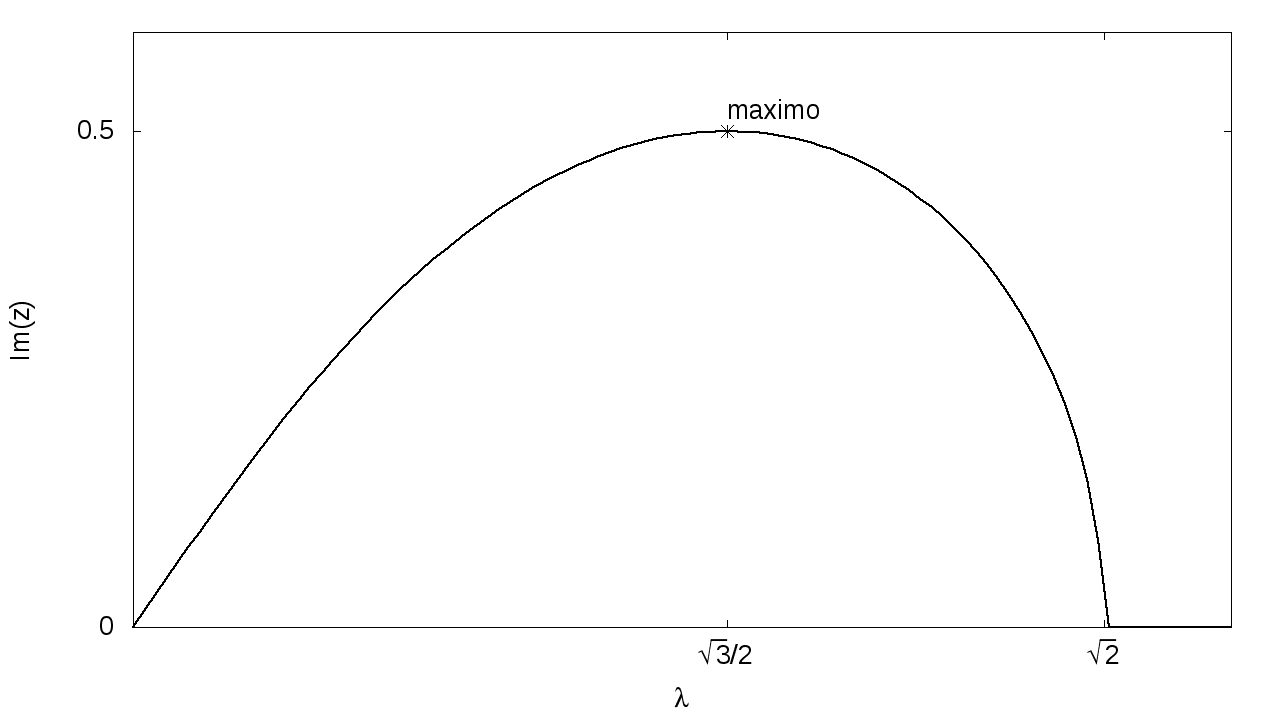
\includegraphics[height=0.3\paperheight]{grafica_misma_omega_contrarias.png}
\caption{Tasa de crecimiento para dos especies con misma $\omega_{p\sigma}^2$ pero con velocidades de signo contrario.}
\label{fig:misma_omega_tasa_de_crecimiento}
\end{figure}
\section{Caso misma $\boldsymbol{\omega_{p\sigma}}$ con una especie incidente y la otra estacionaria.}
La relación de dispersión para este caso es muy similar a la ecuación \ref{dispersion_ep_adimensional}, el único cambio se da en recordar que una de las especies tiene velocidad cero, por lo tanto se tiene:
\begin{equation}
\label{eq:misma_omega_reposo}
1 = \frac{1}{z^2} + \frac{1}{(z-\lambda)^2}
\end{equation}
Al igual que el caso de dos especies con misma $\omega_{p\sigma}^2$ pero con velocidades de signo contrario, la raíz que nos es de interes es la raíz cuya parte imaginaria sea positiva, es decir en donde la perturbación crece exponencialmente con el tiempo. Para resolver la raíz se emplea el cambio de variable $z=x+\frac{\lambda}{2}$ lo que resulta en la siguiente expresión:
\begin{equation}
\label{eq:reducida_misma_reposo}
x^4 - \frac{1}{2}(4 + \lambda^2)x^2 + \frac{1}{16}\lambda^2 (\lambda^2 -8)=0
\end{equation}
La cuál es una ecuación bicuadrática de $x$ que permite entonces escribir:
\begin{equation}
\label{eq:bicuad_misma_reposo}
x^2 = \frac{1}{4}(4 + \lambda^2 \pm 4\sqrt{ \lambda^2 +1})
\end{equation}
De la cual se calcula la raíz para $x$ y se realiza el cambio de variable correspondiente para recuperar una solución en $z$.
\begin{equation}
\label{eq:solucion_misma_reposo}
z = \frac{1}{2}\left(\lambda + \sqrt{4 + \lambda ^2 - 4 \sqrt{1 + \lambda ^2}} \right)
\end{equation}
Los signos de la raíz se escogen para que la parte imaginaria de $z$ sea positiva. Para más detalle sobre la obtención de la raíz véase el apéndice \ref{Ap:raices}.
El siguiente paso es buscar el umbral en donde sucede la inestabilidad y para ello se estudia el lado derecho de la ecuación \ref{eq:misma_omega_reposo} y se observa que tiene dos singularidades $z=0,\lambda$. Aquí, el valor de $\lambda$ determinará el mínimo del lado derecho de \ref{eq:misma_omega_reposo} en el intervalo $(0,\lambda)$, al cual llamaremos $f(z,\lambda)$ por simplicidad. La figura \ref{fig:fz_reposo} ilustra el caso para una cierta $\lambda$, en donde se puede apreciar como el valor de $\lambda$ puede afectar el mínimo en el intervalo $(0,\lambda)$. El mínimo que nos interesa es el de valor $1$ pues ese índica cuando las raíces de ecuación \ref{eq:misma_omega_reposo} empiezan a ser imaginarias. Estrictamente hablando, cuando el mínimo es uno quiere decir que dos de sus raíces reales se vuelven una y es cuando el mínimo es mayor que uno que aparecen raíces imaginarias.
\begin{figure}
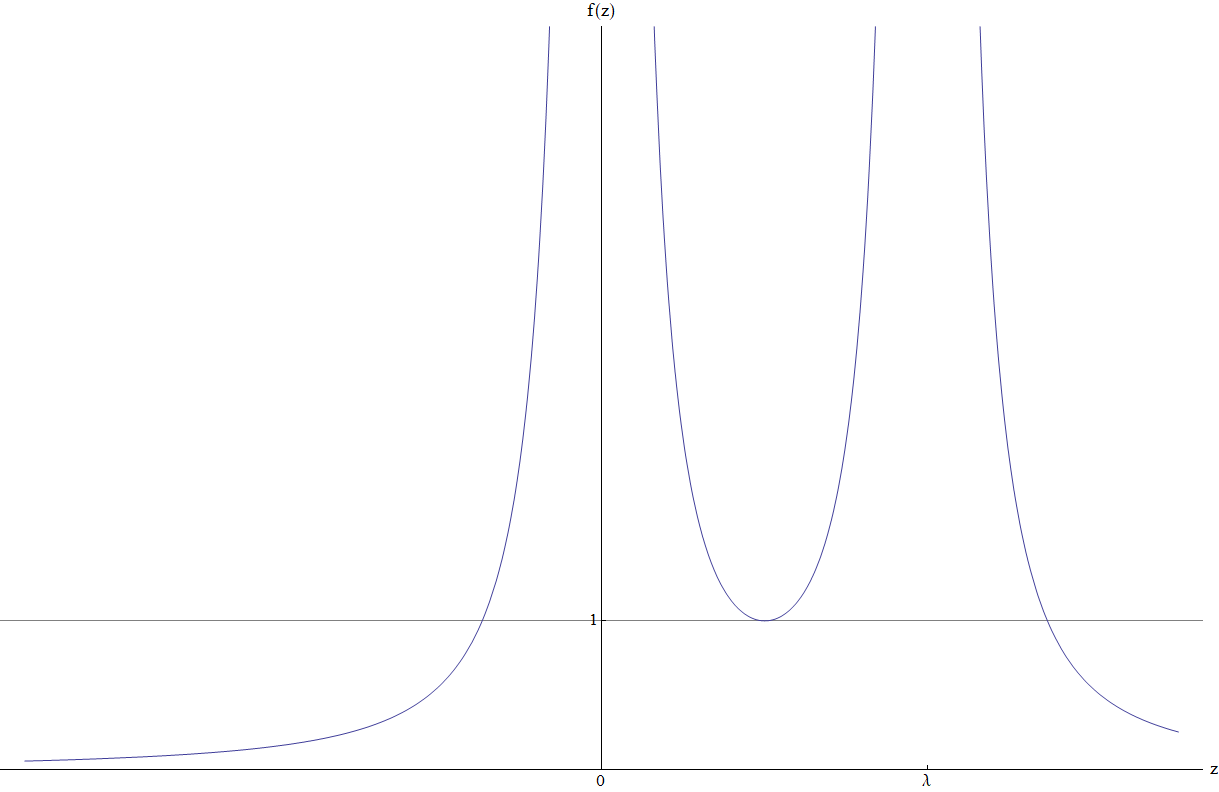
\includegraphics[height=0.3\paperheight]{f_z_reposo.png}
\caption{Gráfica del lado derecho de la ecuación \ref{eq:misma_omega_reposo} para un cierto valor de $\lambda$}
\label{fig:fz_reposo}
\end{figure}
Para encontrar ese umbral se busca entonces para que $\lambda$s el mínimo de $f(z,\lambda)$ es igual a uno. Se empieza entonces por minimizar.
\begin{equation}
\frac{1}{z^3} + \frac{1}{(z-\lambda)^3}=0
\end{equation}
El cual da $z=\lambda / 2$. Que al sustituir en \ref{eq:misma_omega_reposo} y resolver para $\lambda$ da $\lambda = \sqrt{8}$. Por lo que se tiene que el intervalo de inestabilidad es:
\begin{equation}
0 < \lambda < \sqrt{8}
\end{equation}
Para encontrar la máxima tasa de crecimiento se hace uso de que la ecuación \ref{eq:solucion_misma_reposo} representa un número complejo. Basta entonces buscar el máximo de la norma de dicho número. Se tiene entonces:
\begin{equation}
|z|^2 = \frac{1}{4}[\lambda^2 -4 - \lambda^2 + 4(1 + \lambda^2)^{1/2}]
\end{equation}
Donde al observar la ecuación \ref{eq:solucion_misma_reposo} vemos que los términos que le corresponden a la parte imaginaria son $-4 - \lambda^2 + 4(1 + \lambda^2)^{1/2}$. Es decir si $z=x +iy$:
\begin{equation}
y^2= -4 - \lambda^2 + 4(1 + \lambda^2)^{1/2}
\end{equation}
Que al maximizar con respécto de $\lambda$ da:
\begin{equation}
2\lambda -\lambda(1 + \lambda^2)^{1/2} =0
\end{equation}
Y al resolver para $\lambda$ se obtiene
\begin{equation}
\lambda = \sqrt{3}
\end{equation}
Estos valores se pueden apreciar en la figura \ref{fig:misma_omega_tasa_de_crecimiento} que grafica la parte imaginaria de $z$, es decir la correspondiente al crecimiento de la inestabilidad, contra $\lambda$. 
\begin{figure}[!h]
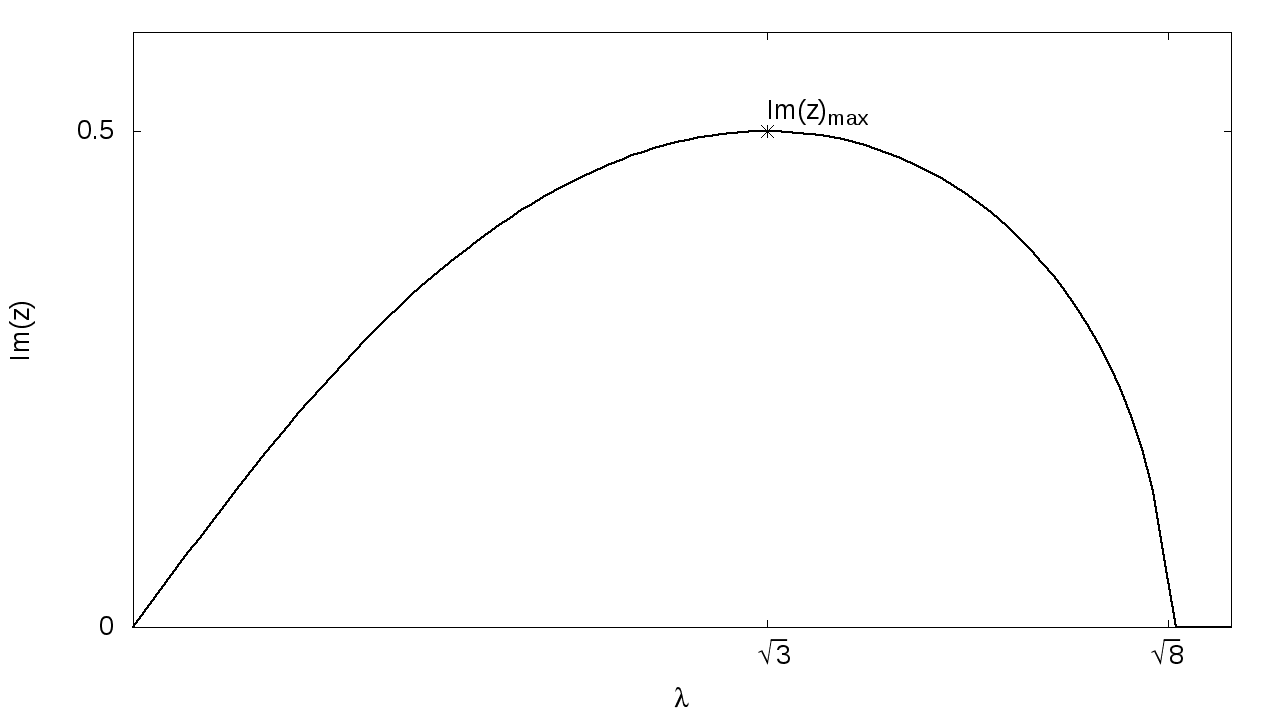
\includegraphics[height=0.3\paperheight]{grafica_misma_omega_reposo.png}
\caption{Tasa de crecimiento para dos especies con misma $\omega_{p\sigma}^2$ pero una de ellas estacionaria.}
\label{fig:misma_omega_reposo}
\end{figure}
Ahora bien regresando a variables físicas se tiene que el umbral de insetabilidad ocurre cuando
\begin{equation}
ku_0 < \sqrt{8} \omega_{p\sigma}
\end{equation}
Y la máxima tasa de crecimiento sucede cuando:
\begin{equation}
ku_0= \sqrt{3} \omega_{p\sigma}
\end{equation}
Y en cuyo caso se tiene
\begin{equation}
\omega = \frac{1}{2} (\sqrt{3} + i)\omega_{p\sigma}
\end{equation}
\section{Generalizando el caso para dos especies con la misma $\boldsymbol{\omega_{p\sigma}}$}
Como se vió en el caso para mismas especies con velocidades opuestas, la relación de dispersión se reduce a una ecuación bicuadrática y de esa manera se encuentran las raíces de la ecuación cuártica. Ésta reducción es posible debido a la simetría del problema. Sin embargo, se tiene que al encontrar las raíces de la ecuación cuártica para el caso de una especie en reposo y otra especie incidente con cierta velocidad arbitraria, también se llega a una ecuación bicuadrática a pesar de no tener la misma simetría que el caso con dos velocidades opuestas. Dicha ecuación bicuadrática aparece como resultado de un cambio de variable $z=x+\lambda /2$, para más detalle véase el apéndice \ref{Ap:raices}. Esto podría sugerir que para dos especies con la misma $\omega_{p\sigma}$ su relación de dispersión siempre se puede reducir a una ecuación bicuadrática con el cambio de variable apropiado. Independientemente de la velocidad que lleve cada especie.\\
Una manera de hacer esto sería partir del caso general y aplicar el cambio de variable sugerido en el apéndice \ref{Ap:raices} para comprobar que se obtiene una ecuación bicuadrática. Sin embargo, otra manera de proceder es partir del caso de una especie en reposo y por medio de un cambio de variable recuperar el caso general.
Se empieza entonces por la relación de dispersión del caso de una especie estacionaria y otra incidente, ambas con la misma $\omega_{p\sigma}$, es decir la ecuación \ref{eq:misma_omega_reposo}.
\begin{equation*}
1 = \frac{1}{z^2} + \frac{1}{(z-\lambda)^2}
\end{equation*}
Si se graficara el lado derecho de la ecuación en función de $z$, véase la figura \ref{fig:fz_reposo}, se observa que los valores de $z$ para los que aparecen raíces complejas se encuentran en el intervalo $(0, \lambda)$. Por otro lado, se puede ver este caso como uno con dos velocidades en donde una de las velocidades resulta ser cero y por lo tanto su $\lambda$ asociada es cero. Se tiene entonces que la distancia entre las dos $\lambda$s es precisamente $\lambda$.\\
Una manera más simple de ver esto es considerando también los otros valores posibles para cada una de las $\lambda$s, recordando que son reales, estos casos son ilustrados en la figura \ref{fig:valores_lambda}.
\begin{figure}[h]
\centering
 \begin{subfigure}[b]{0.4\textwidth}
 	 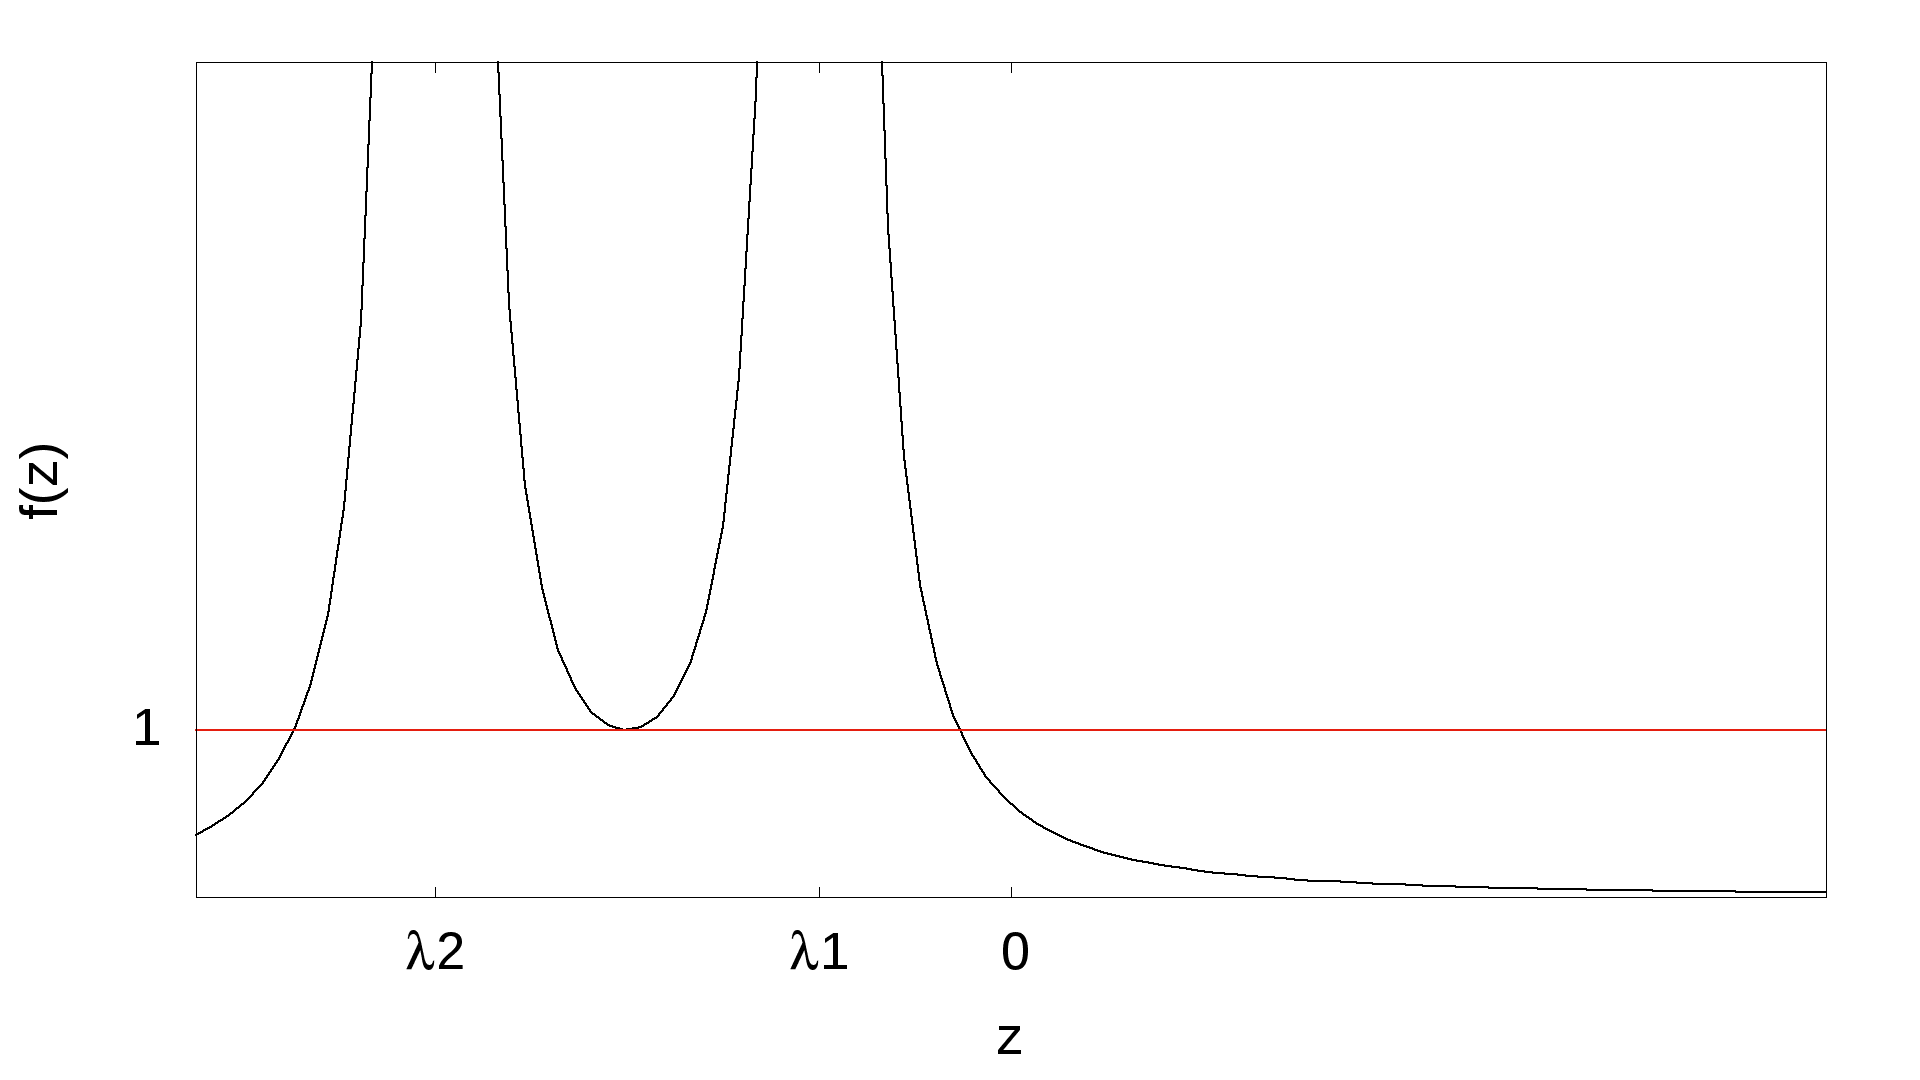
\includegraphics[width=\textwidth]{grafica_lambdas_negativas.png}
 	 \caption{}
 	 \label{fig:lamdas_negativas}
 \end{subfigure}
 
 \begin{subfigure}[b]{0.4\textwidth}
 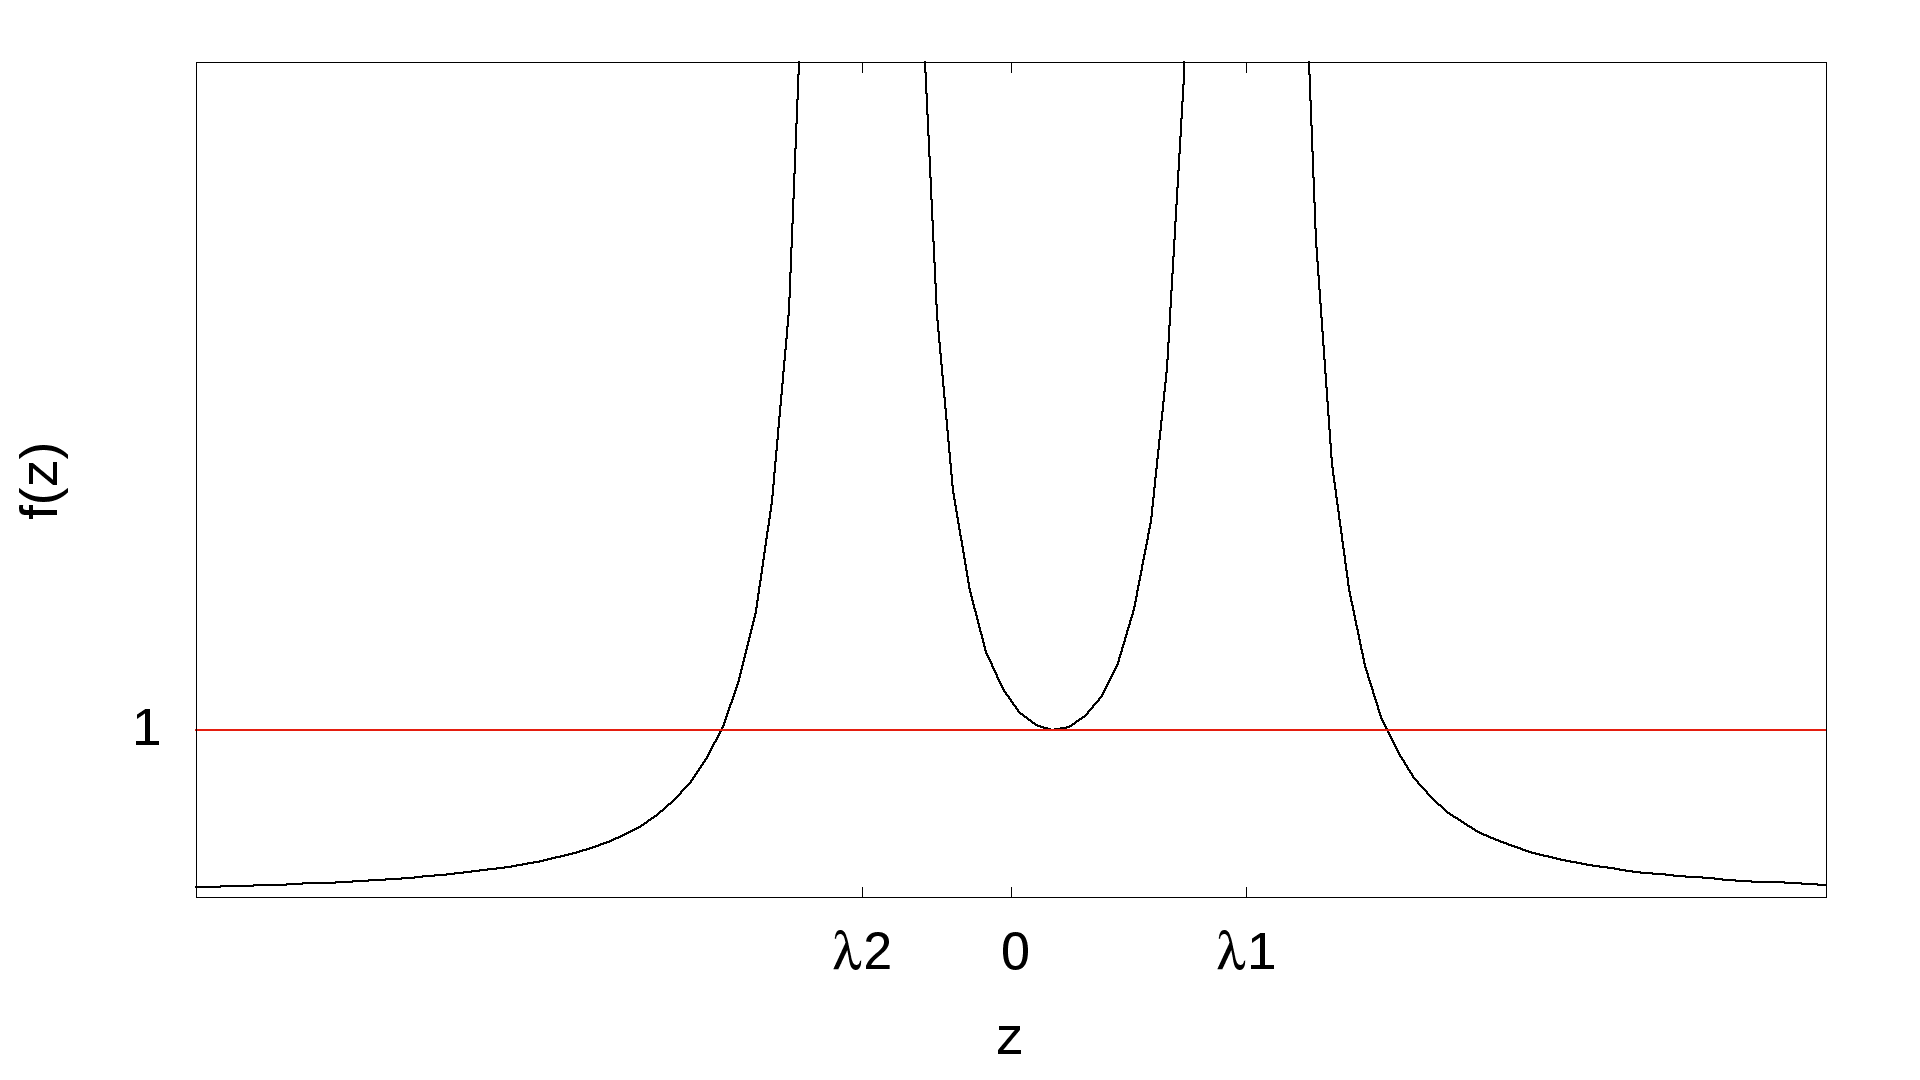
\includegraphics[width=\textwidth]{grafica_lambdas_alternadas.png}
 \caption{}
 \label{fig:lamdas_alternadas}
 \end{subfigure}
 ~
  \begin{subfigure}[b]{0.4\textwidth}
 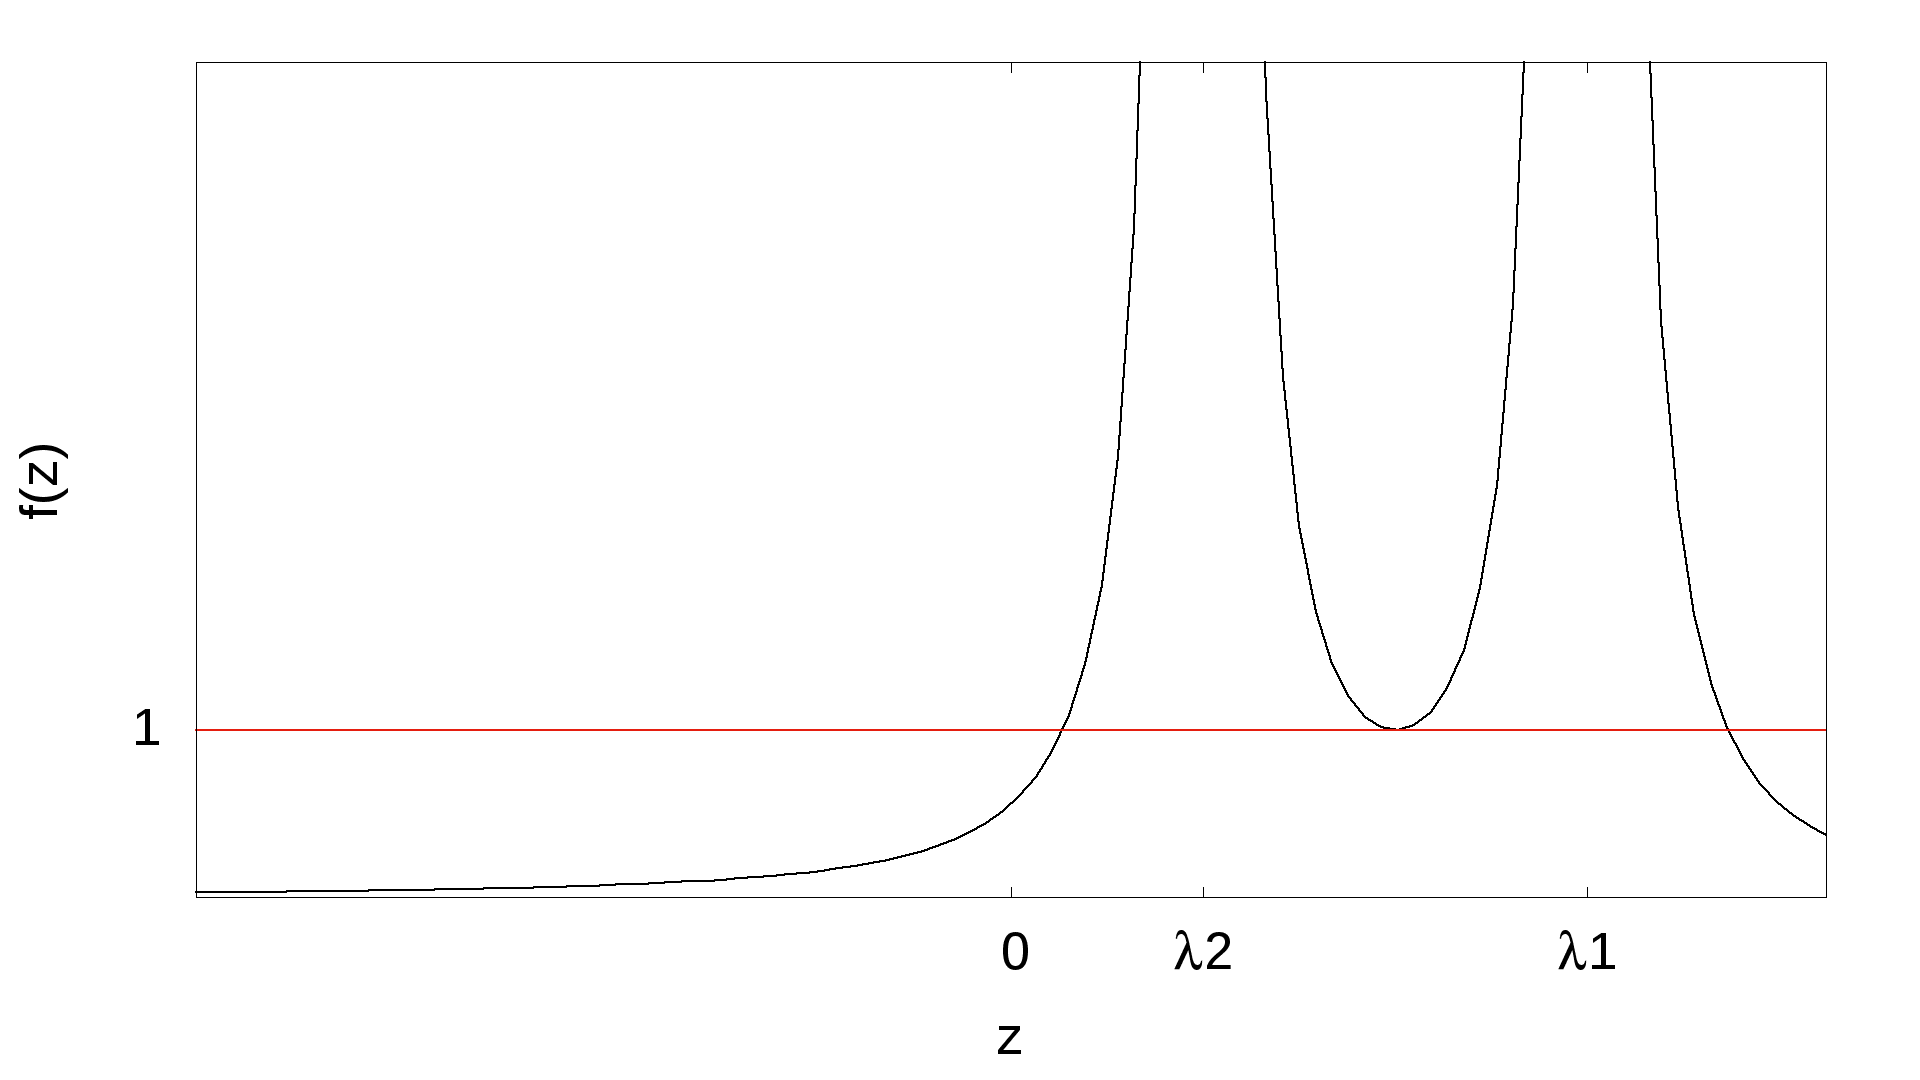
\includegraphics[width=\textwidth]{grafica_lambdas_positivas.png}
  \caption{}
 \label{fig:lamdas_positivas}
 \end{subfigure}
 \caption{Representaciones de los distintos valores que $\lambda_1$ y $\lambda_2$ pueden tomar. Siendo estos cuando ambas son negativas, cuando una es negativa y la otra es positiva y el caso donde ambas son positivas.}\label{fig:valores_lambda}
\end{figure}
Se tiene entonces que se puede definir una distancia $\lambda$ entre $\lambda_1$ y $\lambda_2$ de la forma $\lambda = \lambda_1 - \lambda_2$. La cual permite ver que la ecuación \ref{eq:misma_omega_reposo} es un caso donde $\lambda_2 =0$ y por lo tanto $\lambda_1 = \lambda$. No está de más entonces suponer que si se tiene $\lambda$ constante se puedan recuperar los casos de velocidades opuestas y el de velocidades arbitrarias a partir de una traslación del caso en reposo.\\
Dicha traslación se propone como el cambio de variable $z=z'-\lambda_2$ y recordando que se está tomando $\lambda= \lambda_1 - \lambda_2$ se llega a:
\begin{equation}
\label{eq:misma_omega_general}
1 = \frac{1}{(z'-\lambda_2)^2} + \frac{1}{(z'-\lambda_1)^2}
\end{equation}
Que es el caso general para dos especies con misma $\omega_{p\sigma}$ y velocidades arbitrarias. Lo que la ecuación \ref{eq:misma_omega_general} expone es que el caso de dos velocidades de signo contrario se puede recuperar del caso en reposo ya se haciendo $\lambda_2 = -\lambda_1$ en \ref{eq:misma_omega_general} o realizando el cambio de variable $z=z' +\lambda_1$ y $\lambda= 2\lambda_1$ en \ref{eq:misma_omega_reposo}. Cualquiera de los dos métodos da la expresión:
\begin{equation}
\label{eq:misma_omega_opuestas_cambio}
1 = \frac{1}{(z'+\lambda_1)^2} + \frac{1}{(z'-\lambda_1)^2}
\end{equation}
La cual sabemos se reduce a una ecuación bicuadrática.\\
Del caso de una especie en reposo se tenía que el umbral era:
\begin{equation}
0<\lambda<\sqrt{8}
\end{equation}
Que pasandolo al caso general se tiene:
\begin{equation}
0<\lambda_1 - \lambda_2 <\sqrt{8}
\end{equation}
Por otro lado la máxima tasa de crecmiento sucedía cuando
\begin{equation}
\lambda=\sqrt{3}
\end{equation}
Que resulta ser 
\begin{equation}
\lambda_1 - \lambda_2 = \sqrt{3}
\end{equation}
%\subsection*{Caso con $\omega_{p\sigma}$ diferentes y una especie estacionaria.}
%
\section{Caso para un plasma estacionario y uno incidente}
Este caso consiste en un plasma compuesto por dos especies que se mueven a una velocidad $\overrightarrow{\textbf{u}}_{\sigma 0}$ incidiendo con un plasma estacionario compuesto por las mismas especies. Se trata entonces de un caso de cuatro especies. Cuya relación de dispersión normalizada es de la forma:
\begin{equation}
\label{eq:disp_d-d}
\frac{\epsilon_1}{z^2}+\frac{1}{z^2}+\frac{\epsilon_1}{(z-\lambda)^2}+\frac{1}{(z-\lambda)^2}=1
\end{equation}
Donde $\epsilon_1 = \omega_{p1}/ \omega_{pe}$. Para encontrar el umbral de inestabilidad se realiza el mismo procedimiento de los casos anteriores. Se minimiza la ecuación \ref{eq:disp_d-d} y se resuelve para obtener $z$ en términos de $\lambda$. Que resulta ser $z=\lambda /2$.
\begin{equation}
\frac{\epsilon_1}{z^3}+\frac{1}{z^3}+\frac{\epsilon_1}{(z-\lambda)^3}+\frac{1}{(z-\lambda)^3}=0
\end{equation}
Si se sustituye en \ref{eq:disp_d-d} y se resuelve para $\lambda$ se encuentra entonces que:
\begin{equation}
0 < \lambda < \sqrt{8(1+\epsilon)}
\end{equation}
Para encontrar la máxima tasa de crecimiento se empieza por buscar la raíz del lado derecho de \ref{eq:disp_d-d} que tenga parte imaginaria positiva. Dicha raíz resulta ser:
\begin{equation}
\label{eq:raiz_d-d}
z =\frac{1}{2}\left(\lambda + \sqrt{4 + 4\epsilon + \lambda ^2 -4\sqrt{1+2\epsilon + \epsilon^2+ \lambda^2 + \epsilon \lambda ^2}} \right)
\end{equation}
La cual también se multiplica por su conjugado para así obtener el cuadrado de su componente imaginaria.
\begin{equation}
y^2 = -\left(4 + 4\epsilon + \lambda ^2 -4\sqrt{1+2\epsilon + \epsilon^2+ \lambda^2 + \epsilon \lambda ^2}\right)
\end{equation}
El cual se maximiza con respecto a $\lambda$ y al resolver da $\lambda = \sqrt{3(1 + \epsilon)}$. La cual se sustituye en la ecuación \ref{eq:disp_d-d} para dar:
\begin{equation}
\label{eq:z-max-d-d}
z_{max} = \frac{1}{2}\left(\sqrt{3(1+\epsilon)} + i \sqrt{(1+\epsilon)} \right)
\end{equation}
%Al tratarse de el caso de deuterio, se tiene que $\epsilon = 2.72 \times 10^{-4}$. Que al sustituir en la ecuación \ref{eq:z-max-d-d} da:
%\begin{equation}
%z=0.86614 + 0.50007i
%\end{equation}
%Entonces, el umbral de inestabilidad resulta ser:
%\begin{equation}
%0 < \lambda < 2.82881
%\end{equation}
%Y la máxima tasa de crecimiento sucede cuando $\lambda = 1.73229$.
%Esto se traduce como:
%\begin{equation}
%ku_0 < 2.82881 \omega_{pe}
%\end{equation}
%Para el umbral de inestabilidad.
%\begin{equation}
%ku_0 = 1.73229 \omega_{pe}
%\end{equation}
%Para el valor al cual aparece la máxima tasa de crecimiento.
%\begin{equation}
%\omega = (0.86614 + 0.50007i)\omega_{pe}
%\end{equation}
%Y finalmente la expresión para la frecuencia cuando ésta ocurre. 
La figura \ref{fig:d-d} muestra el comportamiento de la parte imaginaria de $z$ para el caso que se acaba de estudiar.
\begin{figure}
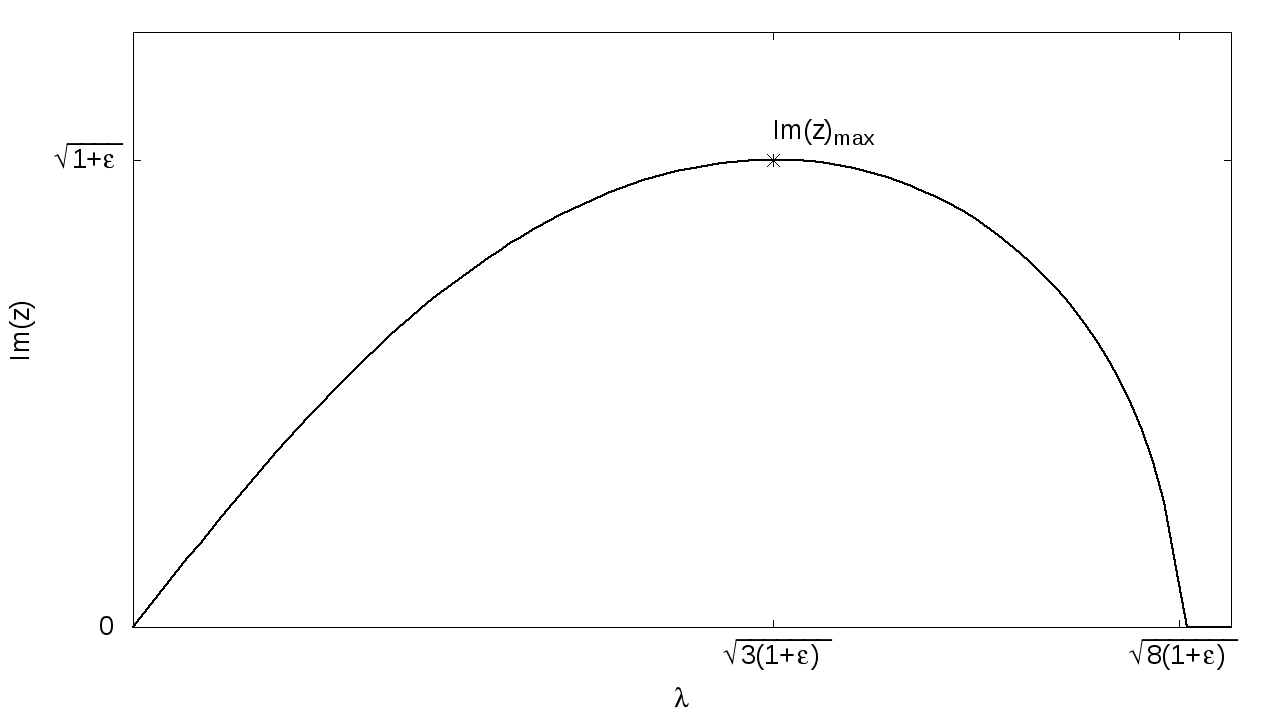
\includegraphics[height=0.3\paperheight]{grafica-d-d-reposo}
\caption{$Im(z)$ en función de $\lambda$, con $\epsilon = 2.72 \times 10^{-4}$ para el caso de un haz de deuterio-electrén incidiendo con un plasma estacionario deuterio-electrón.}
\label{fig:d-d}
\end{figure}
\section{Caso para iones estacionarios y electrones incidentes}
La relación de dispersión para este caso es la siguiente:
\begin{equation}
\label{eq:disp_ion_electron}
\frac{\epsilon}{z^2}+\frac{1}{(z-\lambda)^2}=1
\end{equation}
Donde $z$ y $\lambda$ son las constantes normalizadas de los casos anteriores, mientras que $\epsilon = m_e/m_i$.
Siguiendo el proceso que se ha estado haciendo, lo primero que se busca es el umbral de inestabilidad. Es decir para que valores de $\lambda$ dos raíces reales colapsan a una sola o aparecen raíces complejas. Como ya se había mencionado, esto sucede cuando el mínimo del lado izquierdo de la ecuación \ref{eq:disp_ion_electron} es mayor o igual a la unidad. Si se toma al lado izqueirdo de \ref{eq:disp_ion_electron} como una función $f(z,\lambda)$ y se minimiza se llega a una expresión:
\begin{equation}
\frac{\epsilon}{z^3}+\frac{1}{(z-\lambda)^3}=0
\end{equation}
De donde se busca tener exponentes positivos para $z$ por lo que se manipula para obtener:
\begin{equation}
\frac{z^3}{\epsilon}=-(z-\lambda)^3
\end{equation}
De donde se pueden obtener raíces cúbicas de cada término:
\begin{equation}
\frac{z}{\epsilon ^{1/3}}=-(z-\lambda)
\end{equation}
De la cual se despeja $z$
\begin{equation}
z_{min}=\frac{\epsilon ^{1/3}\lambda}{(1- \epsilon^{1/3})}
\end{equation}
Que es el valor que la variable $z$ debe tener para que el mínimo sea uno. Está $z_{min}$ se puede substituir en la relación de dispersión para llegar al valor de $\lambda$ que buscamos:
\begin{equation}
1=f(z_{min},\lambda)=\frac{(1+\epsilon^{1/3})^3}{\lambda^2}
\end{equation}
Entonces, para que el mímimo sea mayor o igual a uno el valor de $\lambda$ debe ser:
\begin{equation}
\label{eq:umbral_ion_electron}
\lambda \geq (1+\epsilon^{1/3})^{3/2}
\end{equation}
El cual es nuestro umbral de inestabilidad.
El siguiente paso es entonces buscar una raíz para $z$ en la expresión \ref{eq:disp_ion_electron} que describa el crecimiento de una inestabilidad. Sin embargo, a diferencia de los casos anteriores la ecuación \ref{eq:disp_ion_electron} no se reduce a una ecuación bicuadrática al hacer el cambio de variable y por ello el procedimiento para encontrar la raíz es más laborioso. A continuación se muestra a grandes razgos el cálculo de la raíz, el procedimiento se encuentra con mayor detalle en el apéndice \ref{Ap:raices}.\\
Al expandir la ecuación \ref{eq:disp_ion_electron} y realizando el cambio de vairable $z=x+\frac{\lambda}{2}$ se llega a:
\begin{equation}
x^4 + (-\frac{\lambda^2}{2} -\epsilon -1)x^2 + (\epsilon \lambda - \lambda)x + \frac{\lambda^4}{16}-\frac{\epsilon \lambda^2}{4}-\frac{\lambda^2}{4}=0
\end{equation}
De cuyos coeficientes se construye una expresión para el término auxiliar $\alpha_0$ que es de la forma:
\begin{multline}
\alpha_0 = \frac{1}{3}\left(\frac{\lambda^2}{2} + \epsilon + 1 \right)\\
+ \left(\frac{1}{216}\lbrace-\epsilon^3+3\epsilon^2(\lambda^2-1)-
3\epsilon(\lambda^4 +16\lambda^2 +1)+ (\lambda^2 -1)^3\rbrace \right. \\
\left. +\frac{\lambda}{12\sqrt{3}}\lbrace\epsilon [\epsilon^3-3\epsilon^2(\lambda^2 -1)+3\epsilon(\lambda^4 + 7\lambda^2 +1)- (\lambda^2-1)^3]\rbrace^{1/2} \vphantom{\frac{1}{216}}\right)^{1/3}\\
+ \left(\frac{1}{216}\lbrace-\epsilon^3+3\epsilon^2(\lambda^2-1)-
3\epsilon(\lambda^4 +16\lambda^2 +1)+ (\lambda^2 -1)^3\rbrace \right. \\
\left. -\frac{\lambda}{12\sqrt{3}}\lbrace\epsilon [\epsilon^3-3\epsilon^2(\lambda^2 -1)+3\epsilon(\lambda^4 + 7\lambda^2 +1)- (\lambda^2-1)^3]\rbrace^{1/2} \vphantom{\frac{1}{216}}\right)^{1/3}
\end{multline}
Una vez obtenido $\alpha_0$ se puede encontrar entonces una raíz para $x$ cuya parte imaginaria sea postiva y al volver a realizar un cambio de variable se recupera la raíz para $z$.
\begin{equation}
z= \frac{1}{2} \left( \lambda + \sqrt{2\alpha_0} + \sqrt{2\alpha_0 -4 \left(-\frac{1}{2}(\frac{\lambda^2}{2}+\epsilon+1)+\alpha_0 +\frac{\epsilon \lambda - \lambda}{2\sqrt{2\alpha_0}}\right)}\right)
\end{equation}
\section{Amortiguamiento de Landau}
En las secciones anteriores se estudió diferentes casos particulares para la relación de dispersión. Recordando que la forma general está dada por la ecuación \ref{eq_dispersion} que describe un plasma compuesto por distintas especies con velocidades $\overrightarrow{\textbf{u}}_{\sigma 0}$ y frecuencia de plasma $\omega^2_{p \sigma}$.\\
Ahora bien, haciendo la suposición de que se tienen iones en reposo como fondo, la densidad de cada especie se puede escribir entonces como $n_{\sigma 0} = f_{\sigma}n_0$ donde $n_0$ es la densidad de los iones de fondo y $f_{\sigma}$ es la densidad parcial de la especie $\sigma$. De tal manera que la suma de las $f_{\sigma}$ da la unidad. Por lo que la ecuación \ref{eq_dispersion} se puede reescribir como:
\begin{equation}
\label{eq:dispersion_general_1}
1 =\omega^2_{p0}\sum_{\sigma}\frac{f_{\sigma}}{(\omega - \overrightarrow{\textbf{k}}\cdot \overrightarrow{\textbf{u}}_{\sigma 0})^2}
\end{equation}
Donde $\omega^2_{p0}$ es la frecuencia de plasma asociada a la densidad $n_0$. Esta manera alternativa de escribir la relación de dispersión fue simplemente para facilitar la presentación de otra generalización en donde las especies tienen asociadas todas las velocidades y la densidad correspondiente está determinada por una función de distribución $f(v)$, donde el número total de partículas en el intervalo $(v,v+dv)$ está dado por $n_0f(v)dv$. La densidad $f_{\sigma}$ es entonces sustituida por $f(v)dv$ y la suma por unat integral de $-\infty$ a $\infty$.
\begin{equation}
\label{eq:dispersion_general_2}
1= \omega^2_{p0}\int^{\infty}_{-\infty}\frac{f(v)}{(\omega-k v)^2}dv
\end{equation}
Al inetgra por partes:
\begin{equation}
1=\omega^2_{p0}\left(\frac{f(v)}{(\omega - v)k}- \int^{\infty}_{-\infty}\frac{df/dv}{(\omega -k v)k}dv \right)
\end{equation}
Si se asume que $f$ se desvanece en el infinito se tiene entonces:
\begin{equation}
1=-\frac{\omega^2_{p0}}{k}\int^{\infty}_{-\infty}\frac{df/dv}{\omega -k v}dv
\end{equation}
Está forma generalizada presenta un problema ya que hay una singularidad para cuando el valor de $v$ se aproxima al valor de la velocidad de fase de la onda ($\omega/k$).
Para evaluar la integral se hace uso de la teoría de variable compleja, en particular el teorema del residuo y el valor principal de Cauchy.\\
Se reescribe la integral en una forma más conveniente.
\begin{equation}
\label{eq:disp_general_alt}
1=\frac{\omega^2_{p0}}{k^2}\int^{\infty}_{-\infty}\frac{df/dv}{v- \omega /k}dv
\end{equation}
La manera de resolver el problema de la singularidad es tratar a la integral en la ecuación \ref{eq:disp_general_alt} como un problema de integral de contorno, donde el cotorno con el que se trabajará será sobre el eje real de $v$, pues se está trabajando en el plano complejo de $v$, y un semicírculo que pase por debajo del polo $\omega /k$ \cite{hassani2013mathematical}. Se tiene entonces que:
\begin{equation}
\int_{c}\frac{df/dv}{v- \omega /k}dv= \int^{\omega/k -\epsilon}_{-\infty}\frac{df/dv}{v- \omega /k}dv + \int^{\infty}_{\omega/k +\epsilon}\frac{df/dv}{v- \omega /k}dv + \int_{c_0}\frac{df/dv}{v- \omega /k}dv
\end{equation}
Al tomar el límite cuando $\epsilon \rightarrow 0$ los dos primeros términos del lado derecho resultan ser el valor princial de la integral en la ecuación \ref{eq:disp_general_alt}. Por otro lado, se tiene que en en el contorno $c_0$ la magnitud de $v-\omega/k$ es constante por lo que se puede expresar como $v-\omega/k =\epsilon e^{i\theta}$ y $dv= i\epsilon e^{i\theta}d\theta$. De manera que se tiene \cite{hassani2013mathematical}:
\begin{equation}
\int_{c_0}\frac{df/dv}{v- \omega /k}dv = i \pi \left(\frac{df}{dv}\right)_{v=\omega/k}
\end{equation}
Con esto, se reescribe la ecuación \ref{eq:disp_general_alt} como:
\begin{equation}
\label{eq:disp_general_residuo}
1 = \frac{\omega^2_{p0}}{k^2} \left(PV\int^{\infty}_{-\infty}\frac{df/dv}{v- \omega /k}dv + i \pi \left(\frac{df}{dv}\right)_{v=\omega/k}\right)
\end{equation}
Asumiendo el caso donde la velocidad de fase de la onda es mucho mayor que las velocidades en la distribución el valor principal ($PV$) se puede aproximar expandiendo el denominaodr de la integral alrededor de $v=0$, esto da:
\begin{equation}
PV= \frac{1}{\omega}\int^{\infty}_{-\infty} \left(1+\frac{kv}{\omega}+\frac{k^2v^2}{\omega^2}+...\right)\frac{df}{dv}dv
\end{equation}
Y haciendo uso de las propiedades de $f(v)$ como función de distribución \cite{anderson2001tutorial}
\begin{equation}
\int^{\infty}_{-\infty}f(v)dv=1
\end{equation}
\begin{equation}
\int^{\infty}_{-\infty}vf(v)dv=0
\end{equation}
\begin{equation}
\int^{\infty}_{-\infty}v^2f(v)dv=\frac{1}{2}v^2_T
\end{equation}
Se tiene entonces que el valor princial es:
\begin{equation}
PV\int^{\infty}_{-\infty}\frac{df/dv}{v- \omega /k}dv \approx -\frac{k}{\omega^2}\left(1+\frac{3}{2}\frac{k^2v^2_T}{\omega^2}\right)
\end{equation}
Por lo que la relación de dispersión se puede expresar como:
\begin{equation}
\label{eq:disp_var_compleja}
1=\frac{\omega^2_{p0}}{\omega^2}\left(1+\frac{3}{2}\frac{k^2v^2_T}{\omega^2}\right) + i\pi \frac{\omega^2_{p0}}{k^2}\left(\frac{df}{dv}\right)_{v=\omega/k}
\end{equation}
Adicionalmente, si se aproxima al caso $\omega^2 \approx \omega^2_{p0}$ la ecuación \ref{eq:disp_var_compleja} se cambia a:
\begin{equation}
\omega^2=\omega^2_{p0}+\frac{3}{2}k^2v^2_T+i\pi\frac{\omega^4_{p0}}{k^2}\left(\frac{df}{dv}\right)_{v=\omega/k}
\end{equation}
Es de interes entonces la parte imaginaria de $\omega$. Para esto, se recuerda que $\omega/k$ es lo suficientemente grande en comparación con las velocidades de la distribución que la derivada de la función de distribución es lo suficientemente pequeña para realizar una aporximación por series. Adicionalmente, se desprecia la corrección térmica de la parte real \cite{chenintroplasmas}, de manera que se tiene
\begin{equation}
\omega^2 \approx \omega^2_{p0}\left(1+i\pi\frac{\omega^2_{p0}}{k^2}\left(\frac{df}{dv}\right)_{v=\omega/k}\right)
\end{equation}
Al realizar una aproximación en series para encontar $\omega_{im}$ se llega a:
\begin{equation}
\omega_{im}\approx \frac{\pi \omega^2_{p0}}{2k^2}\left(\frac{df}{dv}\right)_{v=\omega/k}
\end{equation}
Ahora bien si $f(v)$ es una distribución maxwelliana entonces $f(v) \propto exp(-v^2/v^2_T)$, es decir una función decreciente en la velocidad por lo que su derivada evaluada en $\omega/k$ es negativa y entonces $\omega_{im}$ representa un amortiguamiento en la onda.
A este amortiguamineto se le conoce como amortiguamiento de Landau, cuyo origen resulta evidente si se recuerda que la suposición de una velocidad de fase lo suficientemente grande inplica que las especies se mueven a una velocidad más lenta y por lo tanto la transferencia de energía es desde la onda hacia las partículas.
\onlyinsubfile{\bibliographystyle{unsrt}}
\onlyinsubfile{\bibliography{../referencias}}
\end{document}